\documentclass[a4paper,12pt]{report}
\usepackage{times}
\usepackage{graphicx}
\begin{document}
	\begin{center}
		\textbf{NETACODE -A SOFTWARE COMPANY VISITING REPORT}\\
		\begin{flushleft}
			The report is visiting a software company for \textbf{Course tittle:Information System Design with industrial attachment Sessional} Course and \textbf{Course Code:CSE 3210} in Computer Science and Engineering.\\
		\end{flushleft}
				by\\	
			Mst.Habiba Hena Sumi(200101070)\\Most.Jannat-Ul-Ferdoush(200101068)\\Md.Talath Un Nabi(200101076)\\Ferdous Tahsin(200101079)\\
			
			\begin{figure}[h]
				\centering
				\includegraphics[width=0.4\linewidth]{"images (1)"}
				\label{fig:images-1}
			\end{figure}
		
		\vspace{1 cm}
			Submited To:\\
			Teacher name:Ananna Hoque Shathi\\
			Department of Computer Science and Engineering(CSE)\\
			Bangladesh Army University of Science and Technology(BAUST)\\
			
		\end{center}
	
	\begin{flushright}
		\vspace{3 cm}
		...............................................\\
		signature of the teacher
	\end{flushright}
\newpage
\tableofcontents
\listoffigures
\listoftables
\newpage

\chapter{Systems Concepts and the Information Systems Environment}
\section{INTRODUCTION}
 System analysis and design is a process that many companies use to evaluate particular business situations and develop ways to improve them through more optimal methods.\\
 
\section {Characteristic of System:}
\textbf{Organization}
Their organization has a branch in Dinajpur district. Netacode is a multinational software company. Main office in Dhaka in Bangladesh. Their organizations are certainly very beautiful. 4 storied building and their number of rooms is 7.\\

\textbf{Interaction}
It is defined by the manner in which the components operate with each other.For example, in an organization,purchasing department must interact with production department and payroll with personnel department.\\

\textbf{Interdependence}
Interdependence means how the components of a system depend on one another. For proper functioning, the components are coordinated and linked together according to a specified plan. \\

\textbf{Integration}
Integration is concerned with how a system components are connected together. It means that the parts of the system work together within the system even if each part performs a unique function.\\

\textbf{Central Objective}
The objective of system must be central. It may be real or stated. It is not uncommon for an organization to state an objective and operate to achieve another.\\
\begin{figure}[h]
	\centering
	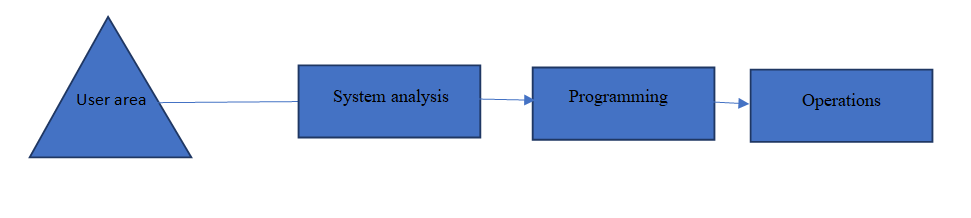
\includegraphics[width=0.7\linewidth]{1}
	\caption{Task Interdependence in a Computer – Based Subsystem }
	\label{fig:1}
\end{figure}
\section{Elements of System}
\textbf{Outputs and Inputs}
\begin{itemize}
	\item 	The main aim of a system is to produce an output which is useful for its user.
	\item 	Inputs are the information that enters into the system for processing.
	\item 	Output is the outcome of processing.
\end{itemize}
\textbf{Processor(s)}
\begin{itemize}
	\item 	The processor is the element of a system that involves the actual transformation of input into output.
	\item 	It is the operational component of a system. Processors may modify the input either totally or partially, depending on the output specification.
\end{itemize}
\textbf{control}
\begin{itemize}
	\item The control element guides the system.
	\item	It is the decision–making subsystem that controls the pattern of activities governing input, processing, and output.
\end{itemize}
\textbf{Feedback}
\begin{itemize}
	\item Feedback provides the control in a dynamic system.
	\item	Positive feedback is routine in nature that encourages the performance of the system.
	\item	Negative feedback is informational in nature that provides the controller with information for action.
\end{itemize}
\textbf{Environment}
\begin{itemize}
	\item	The environment is the “supersystem” within which an organization operates.
	\item	It is the source of external elements that strike on the system.
\end{itemize}
\textbf{Boundaries and Interface}
\begin{itemize}
	\item	A system should be defined by its boundaries. Boundaries are the limits that identify its components, processes, and interrelationship when it interfaces with another system.
	\item	Each system has boundaries that determine its sphere of influence and control.
\end{itemize}
\begin{figure}[h]
	\centering
	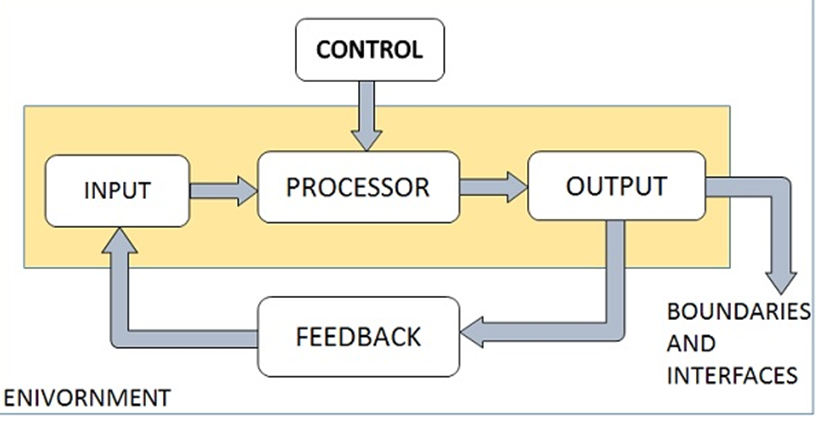
\includegraphics[width=0.7\linewidth]{2}
	\label{fig:2}
\end{figure}
\section{Types of Systems}
The systems can be divided into the following types 
\textbf{Physical or Abstract Systems}
\begin{itemize}
	\item	Physical systems are tangible entities. We can touch and feel them.
	\item	Physical System may be static or dynamic in nature. For example, desks and chairs are the physical parts of computer center which are static. A programmed computer is a dynamic system in which programs, data, and applications can change according to the user's needs.
	\item	Abstract systems are non-physical entities or conceptual that may be formulas, representation or model of a real system.
\end{itemize}
\textbf{Open or Closed Systems}
\begin{itemize}
	\item	An open system must interact with its environment. It receives inputs from and delivers outputs to the outside of the system. For example, an information system which must adapt to the changing environmental conditions.
	\item	A closed system does not interact with its environment. It is isolated from environmental influences. A completely closed system is rare in reality.
\end{itemize}
\begin{figure}[h]
	\centering
	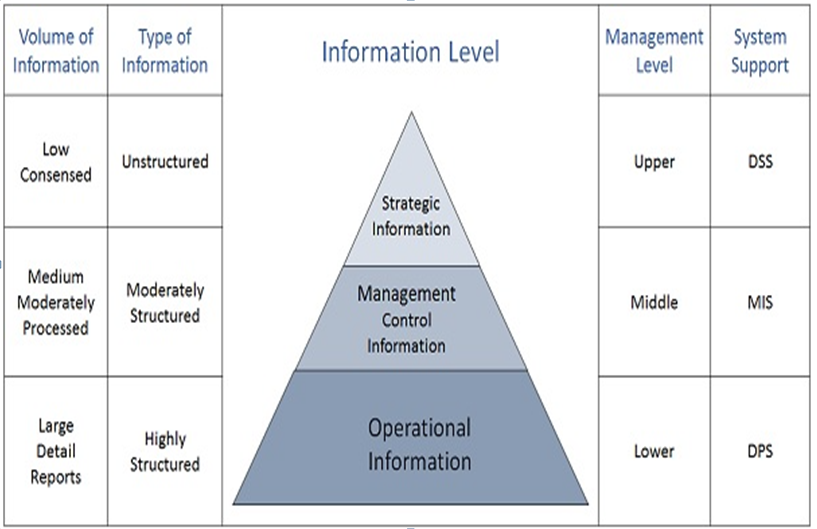
\includegraphics[width=0.7\linewidth]{3}
	\caption{Categories of information related to managerial levels and the decision managers make.}
	\label{fig:3}
\end{figure}
\newpage
\textbf{Goals}\\
To provide trouble-free, customer-focused, reliable, and affordable web hosting services. WE simply want
to continue to operate a profitable web hosting company that makes customers happy. Since the
beginning, we have backed our rock solid hosting solutions and top-notch infrastructure with the best
customer service and technical support. A common feeling about the technology field is it's all about
machines, yes, It does take machines but, Host Pair also knows it takes good people to run a well-oiled
machine. Yes, a successful business needs to be committed to client solutions, innovation, creativity, and
a warm, caring attitude to all of our customers' business needs. We don't just provide 24x7 support. We
really do listen and care.
\end{document}
